\documentclass[english]{SPFShortReport}
\usepackage{subfigure}
\usepackage{spfFigures}
\usepackage{longtable}
\usepackage{url}
\usepackage{gensymb}
\usepackage[yyyymmdd,hhmmss]{datetime}
\reportName{Python calculation for heat pump HP06L-K-BC}
\reportSubName{Parametric Heat Pump calculation} 
\reportDate{\today \hspace{0.1cm} at: \currenttime \hspace{0.1cm} h} 
\author{Dani Carbonell}
\address{dani.carbonell@solarenergy.ch}
\begin{document}
\begin{table}[!ht]
\begin{small}
\caption{Fitted coefficients for the heat pump.}
\begin{center}
\resizebox{12cm}{!} 
{
\begin{tabular}{l | c c } 
\hline
\hline
Coefficient &Description & \\ 
 & &$[kW]$\\ 
\hline
$PQ_{1}$ & \emph{$1^{st}$ condenser polynomial coefficient}  & 5.7318e+00    \\ 
$PQ_{2}$ & \emph{$2^{st}$ condenser polynomial coefficient}  & 6.0957e+01    \\ 
$PQ_{3}$ & \emph{$3^{st}$ condenser polynomial coefficient}  & 2.8445e+01    \\ 
$PQ_{4}$ & \emph{$4^{st}$ condenser polynomial coefficient}  & 9.5982e+00    \\ 
$PQ_{5}$ & \emph{$5^{st}$ condenser polynomial coefficient}  & 5.1491e+01    \\ 
$PQ_{6}$ & \emph{$6^{st}$ condenser polynomial coefficient}  & -1.5297e+02    \\ 
\hline
$PCOP_{1}$ & \emph{$1^{st}$ COP polynomial coefficient}  & 8.4084e+00    \\ 
$PCOP_{2}$ & \emph{$2^{st}$ COP polynomial coefficient}  & 7.1520e+01    \\ 
$PCOP_{3}$ & \emph{$3^{st}$ COP polynomial coefficient}  & -3.6218e+01    \\ 
$PCOP_{4}$ & \emph{$4^{st}$ COP polynomial coefficient}  & -2.6541e+02    \\ 
$PCOP_{5}$ & \emph{$5^{st}$ COP polynomial coefficient}  & 6.6681e+01    \\ 
$PCOP_{6}$ & \emph{$6^{st}$ COP polynomial coefficient}  & 1.9120e+01    \\ 
\hline
$\dot m_{cond}$ & 1200.00 $[kg/h]$\\ 
$\dot m_{evap}$ & 3000.00 $[kg/h]$\\ 
\hline
$COP_{nom}$ (B0W35)& 4.00 \\ 
$Q_{c,nom}$ (B0W35)& 6.40 kW\\ 
$COP_{nom}$ (B2W35)& 4.28 \\ 
$Q_{c,nom}$ (B2W35)& 6.81 kW\\ 
$COP_{nom}$ (B10W35)& 5.44 \\ 
$Q_{c,nom}$ (B10W35)& 8.48 kW\\ 
\hline
\hline
\end{tabular}
}
\label{CoefTable}
\end{center}
\end{small}
\end{table}
\begin{table}[!ht]
\begin{small}
\caption{Predicting results of the heat pump.}
\begin{center}
\resizebox{12cm}{!} 
{
\begin{tabular}{l | c c c c c c c c c c c } 
\hline
\hline
$T_{evap,in}$ &$T_{evap,out}$ &$T_{cond,in}$ &$T_{cond,out}$ &$COP$ &$Q_{cond}$ &$Q_{evap}$ &$W_{comp}$ &$\dot m_{cond}$ &$\dot m_{evap}$ &$\Delta T_{evap}$ &$\Delta T_{cond}$ \\ 
$^oC$ &$^oC$ &$^oC$ &$^oC$ &$[-]$ &$[kW]$ &$[kW]$ &$[kW]$ &kg/h &kg/h &K &K\\ 
\hline
-7.00 & -8.99 & 47.02 & 50.00 & 1.92 & 4.17 & 2.00 & 2.17 & 1200 & 3000 & 2.0 & 3.0\\ 
-7.00 & -7.88 & 55.05 & 57.50 & 1.35 & 3.42 & 0.89 & 2.54 & 1200 & 3000 & 0.9 & 2.5\\ 
-7.00 & -6.29 & 63.23 & 65.00 & 0.78 & 2.47 & -0.71 & 3.19 & 1200 & 3000 & -0.7 & 1.8\\ 
7.00 & 2.16 & 44.90 & 50.00 & 3.14 & 7.12 & 4.85 & 2.27 & 1200 & 3000 & 4.8 & 5.1\\ 
7.00 & 3.44 & 52.88 & 57.50 & 2.24 & 6.46 & 3.57 & 2.88 & 1200 & 3000 & 3.6 & 4.6\\ 
7.00 & 5.55 & 60.96 & 65.00 & 1.35 & 5.64 & 1.45 & 4.19 & 1200 & 3000 & 1.4 & 4.0\\ 
\hline
\hline
\end{tabular}
}
\label{ResultsTable}
\end{center}
\end{small}
\end{table}
\begin{figure}[!ht]
\begin{center}
\includegraphics[width=1\textwidth]{C:/Daten/OngoingProject/TRNSYS-Polysun/HeatPumpFit/AirToWater/Heliotherm/HP06L-K-BC/HP06L-K-BC-Cop.pdf}
\caption{COP Results for the heat pump at the selected points}
\label{COPFig}
\end{center}
\end{figure}
\begin{figure}[!ht]
\begin{center}
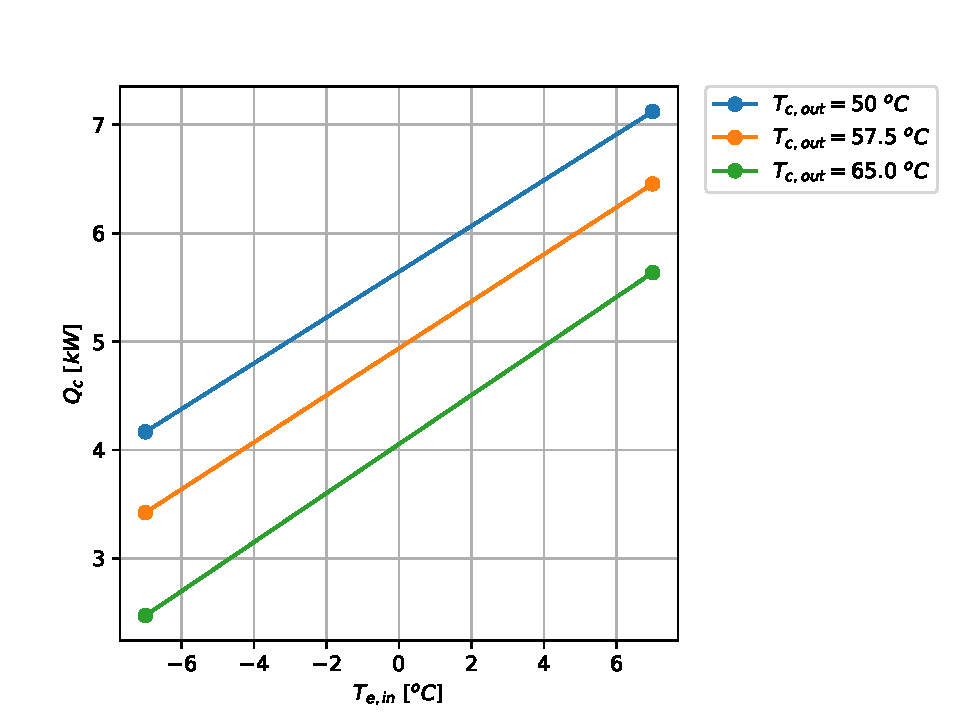
\includegraphics[width=1\textwidth]{C:/Daten/OngoingProject/TRNSYS-Polysun/HeatPumpFit/AirToWater/Heliotherm/HP06L-K-BC/HP06L-K-BC-Qc.pdf}
\caption{$Q_c$ Results for the heat pump at the selected points}
\label{QcFig}
\end{center}
\end{figure}
\end{document}
